\section{Alattin Approach}
\label{sec:framework}

\begin{figure}[t]
\begin{CodeOut}
\begin{alltt}
01:public Object evaluate(Object val) \{ ...
02:\hspace*{0.2in}if (val != null && 
\hspace*{1.3in}val instanceof Collection) \{
03:\hspace*{0.4in}Collection coll = (Collection) val;
04:\hspace*{0.4in}Iterator i = coll.iterator(); 
05:\hspace*{0.4in}if(!coll.isEmpty()) \{
06:\hspace*{0.6in}for (; i.hasNext();) \{
07:\hspace*{0.8in}Object obj = i.next(); 
08:\hspace*{0.8in}if(obj instanceof Node) \{
09:\hspace*{1.0in}Node node = (Node) obj;
10:\hspace*{1.0in}//...
11:\hspace*{0.8in}\} \} \} \}
12:\hspace*{0.2in}return new Double(sum);
13:\}
\end{alltt}
\end{CodeOut}\vspace{-1ex}
\Caption{\label{fig:csecodeexample} A code example using
\CodeIn{Iterator.next} gathered from Google code search.}\vspace{-4ex}
\end{figure}

Our Alattin approach accepts an application under analysis and detects neglected conditions around APIs reused by the application. More specifically, Alattin scans the application and gathers APIs reused by the application. Alattin uses ImMiner to mine patterns that serve as programming rules in reusing those APIs. Then Alattin detects violations of these programming rules. In summary, Alattin includes four major phases. In Phase 1, Alattin gathers relevant code
examples that reuse APIs. In Phase 2, Alattin analyzes gathered code examples to generate pattern candidates suitable for mining. In Phase 3, Alattin applies ImMiner on pattern candidates to mine patterns. In Phase 4, Alattin detects violations of mined patterns in the application under analysis. We next explain each phase in detail. We use notations $C_i$ and $F_i$ to denote a class or a method used by the application under analysis, respectively.

\Comment{\begin{figure}[t]
\centering
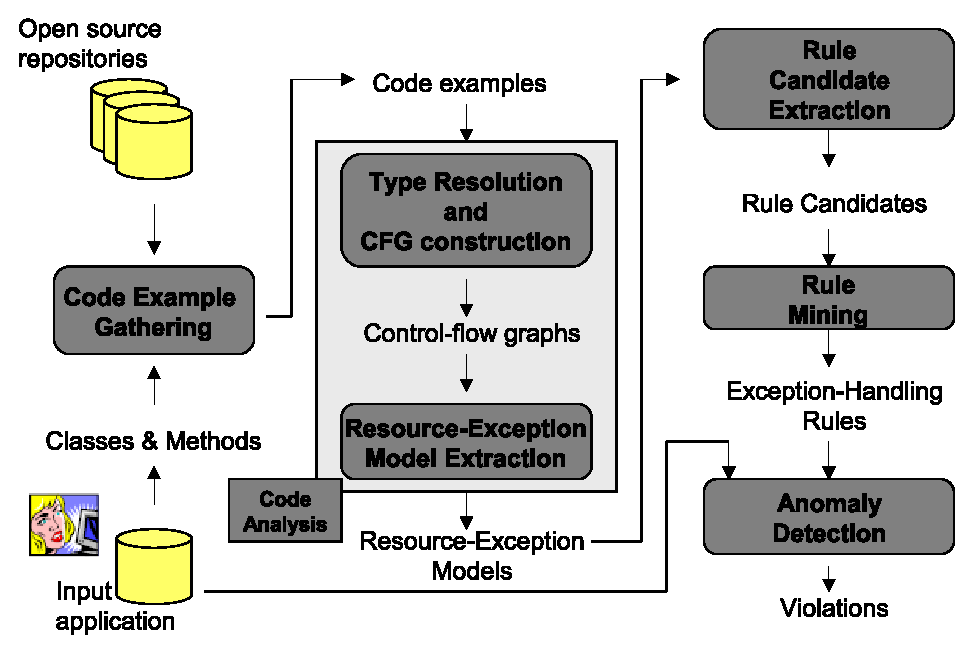
\includegraphics[scale=0.55,clip]{figs/architecture1.eps}\vspace*{-3ex}
\caption{Overview of Alattin framework} \label{fig:architecture}
\vspace*{-4ex}
\end{figure}
}
%--------------------------------------------------------------------------
\subsection {Phase 1: Gathering Code Examples}
\label{sec:cse}

Our approach gathers code examples that include information on how to reuse classes and methods used by the application under analysis. Gathering code examples from a small number of project code bases often cannot surface out many programming rules as common patterns. The primary reason is that there are often too few data points in a small number of code bases to support the mining of desirable patterns. This phenomenon is reflected on empirical results reported by existing mining approaches~\cite{Zhenmin2005PRMiner, chang07:finding}: often a relatively small number of real programming rules mined from one or a few huge code bases. 

To address the preceding issues of a limited number of code bases, Alattin collects code examples from existing open source repositories through code search engines (CSE) such as Google code search~\cite{GCSE} and Koders~\cite{KODERS}. These code search engines are primarily used by programmers in searching for relevant code examples from available open source projects on the web. As these CSEs can serve as powerful resources of open source code, these CSEs can be exploited for other tasks such as detecting violations in applications that reuse existing open source projects. Our approach uses a CSE to gather relevant code examples and mines gathered code examples to detect violations in an application under analysis.

To collect code examples through a CSE, Alattin constructs queries for each $C_i$ and $F_i$. For example, Alattin constructs query of the form ``\CodeIn{lang:java Iterator next}'' to collect code examples that invoke the \CodeIn{next} method of the \CodeIn{Iterator} class. More specifically, our queries include the names of the class and method along
with the language type. Alattin stores gathered code examples in the local file system for further analysis. 
Alattin uses Google code search (GCSE)~\cite{GCSE} for collecting relevant code examples with two main reasons: (1) GCSE provides client libraries that can be used by other tools to interact with and (2) GCSE has public forums that provide good support. However, our approach is independent of GCSE and can leverage any other CSE to gather relevant code examples.
%--------------------------------------------------------------------------
\subsection {Phase 2: Generating Pattern Candidates}
\label{sec:codeanalyzer}

In Phase 2, Alattin analyzes gathered code examples statically to generate pattern candidates suitable for mining. These pattern candidates include condition checks that are performed before and after invoking an $F_i$ method. To identify these condition checks on method calls, Alattin has to associate condition checks in the conditional expressions of \CodeIn{If} or \CodeIn{While} statements with the related method calls. We use the \CodeIn{Iterator.next} method and its relevant code example in Figure~\ref{fig:csecodeexample} as a running example for explaining Phase 2. 

Alattin includes two sub-phases in Phase 2: CFG construction and traversal. In the CFG construction sub-phase, Alattin constructs CFGs for each code example with two kinds of nodes: control ($CT$) and non-control ($NT$) nodes. Control nodes represent control-flow statements such as \emph{if}, \emph{while}, and \emph{for}, which control the flow of the program execution. Non-control nodes represent other statements such as method calls or type casts. For example, Statement 5 in the code example (Figure~\ref{fig:csecodeexample}) is a control node and Statement 9 is a non-control node. When encountering a control node, say $CT_i$ ($i$ indicates the statement id), Alattin also extracts all variables, say \{$V_1$, $V_2$, ..., $V_n$\}, that participate in the conditional expression of that node and the condition checks on those variables. For example, the control node $CT_2$ includes the \{(\CodeIn{val}, \CodeIn{null-check}), (\CodeIn{val}, \CodeIn{instance-check})\} pairs. If the control node includes comparisons with expressions such as method calls, our approach stores those method calls also as additional information within the control node. When encountering a non-control node such as a method call, Alattin extracts variables such as \{\CodeIn{receiver}, \CodeIn{argument1}, ..., \CodeIn{argumentN}\} associated with the method call.

In the CFG traversal sub-phase, Alattin associates gathered condition checks with their related method calls such as \CodeIn{Iterator.hasNext}. The traversal phase includes two kinds of traversals: backward and forward. Alattin performs a backward traversal from the call site such as $NT_7$ of the $F_i$ method to collect condition checks on the receiver and argument objects preceding the call site. Similarly, Alattin performs a forward traversal to collect condition checks on the receiver and return objects after the call site of the $F_i$ method. In each traversal, Alattin exploits program dependencies for associating condition checks with method calls. Failing to consider these program dependencies may result in programming rules that are not semantically related as shown in the limitations of the PR-Miner~\cite{Zhenmin2005PRMiner} and DynaMine~\cite{livshits05dynamine} approaches. To exploit program dependencies, Alattin uses the concept of \emph{dominance} with a combination of \emph{control-flow} and \emph{data-flow} dependencies.

\textbf{Definition}: \emph{A node $N$ \textbf{dominates} another node $M$ in a control flow graph (represented as N dom M) if every path from the starting node of the CFG to $M$ includes $N$.}\\

Initially, Alattin identifies the dominant $CT_i$ nodes for each $NT_k$ node. For example, the control node $CT_6$ dominates the non-control node $NT_7$. Alattin computes the intersection between the variable set associated with the $CT_i$ node, say \{$V_1$, $V_2$, ..., $V_n$\}, and the receiver or argument variables of the $NT_k$ node, say \{\CodeIn{receiver}, \CodeIn{argument1}, ..., \CodeIn{argumentN}\}. If the intersection  \{$V_1$, $V_2$, ..., $V_n$\} $\cap$ \{\CodeIn{receiver}, \CodeIn{argument1}, ..., \CodeIn{argumentN}\} $\neq$ $\emptyset$, Alattin checks whether the $NT_k$ node is dependent on the $CT_i$ node, i.e., whether there exists at least one variable of $NT_k$ node involved in the $CT_i$ node and is not redefined in the path between $CT_i$ and $NT_k$ nodes. If the $NT_k$ node is dependent on the $CT_i$ node, Alattin adds the condition check to the pattern candidate. For example, the extracted condition check for nodes $CT_6$ and $NT_7$ in the code example is ``\CodeIn{boolean-check} on return of \CodeIn{Iterator.hasNext} before \CodeIn{Iterator.next}'', which indicates that a \CodeIn{boolean-check} must be done on the return variable of the \CodeIn{hasNext} method before the call site of \CodeIn{Iterator.next}.  In our experience, we found that there can be various code examples without any condition checks around an $F_i$ method. Failing to consider these code examples can assign incorrect support values to mined patterns. To address this issue, we add an \emph{Empty Pattern Candidate} to the input database ISD for each such code example.
%--------------------------------------------------------------------------
\subsection {Phase 3: Mining Alternative Patterns}
\label{sec:patternminer}

In Phase 3, Alattin uses the ImMiner algorithm to mine both balanced and imbalanced patterns from pattern candidates. Alattin applies ImMiner on pattern candidates of each $F_i$ method individually. The reason is that if we apply ImMiner on all pattern candidates together, the patterns related to an $F_i$ method with a few pattern candidates can be missed due to patterns (related to other $M_j$ methods) with a large number of pattern candidates. 

We apply ImMiner on the pattern candidates of each $F_i$ method in two steps. In Step 1 of mining, ImMiner computes frequent patterns by applying frequent itemset mining. We used a \emph{min\_sup} threshold value of $0.4$. Consider that Step 1 resulted in a pattern ``$P_1$ \textbf{or} $P_2$ \textbf{or} $\ldots$ \textbf{or} $P_i$''. In Step 2, for each frequent alternative, ImMiner gathers the pattern candidates that do not support the alternative and mines infrequent alternative patterns. We use an \emph{alt\_sup} threshold value of $0.2$. These two threshold values are based on our initial empirical experience presented in Section~\ref{sec:thresholds}. At the end of Step 2, ImMiner generates patterns of the form  ``$P_1$ \textbf{or} $P_2$ \textbf{or} $\ldots$ \textbf{or} $P_i$ \textbf{or} $\hat{A_1}$ \textbf{or} $\hat{A_2}$ \textbf{or} $\ldots$ \textbf{or} $\hat{A_j}$'' for each $F_i$ method. In this mined pattern, there are $i$ frequent alternatives and $j$ infrequent alternatives. In our approach, there is no restriction on the number of alternatives (either frequent or infrequent) within a pattern. However, each mined pattern includes at least one frequent alternative.

%--------------------------------------------------------------------------
\subsection{Phase 4: Detecting Neglected Conditions}
\label{sec:anamolydetector}

In Phase 4, Alattin detects violations of mined patterns in an application under analysis statically. More specifically,
Alattin gathers condition checks around each call site of an $F_i$ method in the application under analysis. As each mined pattern contains several alternatives of using the $F_i$ method, Alattin verifies whether a call site of the $F_i$ method in the application under analysis satisfies at least one alternative of the mined pattern. If the gathered condition checks in the application under analysis do not satisfy any of the alternatives of the mined pattern, Alattin reports a violation. \Comment{TODO: To define when we consider that a call site does not satisfy the mined pattern.} For each detected violation, Alattin assigns a support value as the same value as the support value of the associated mined pattern used to detect the violation. 
